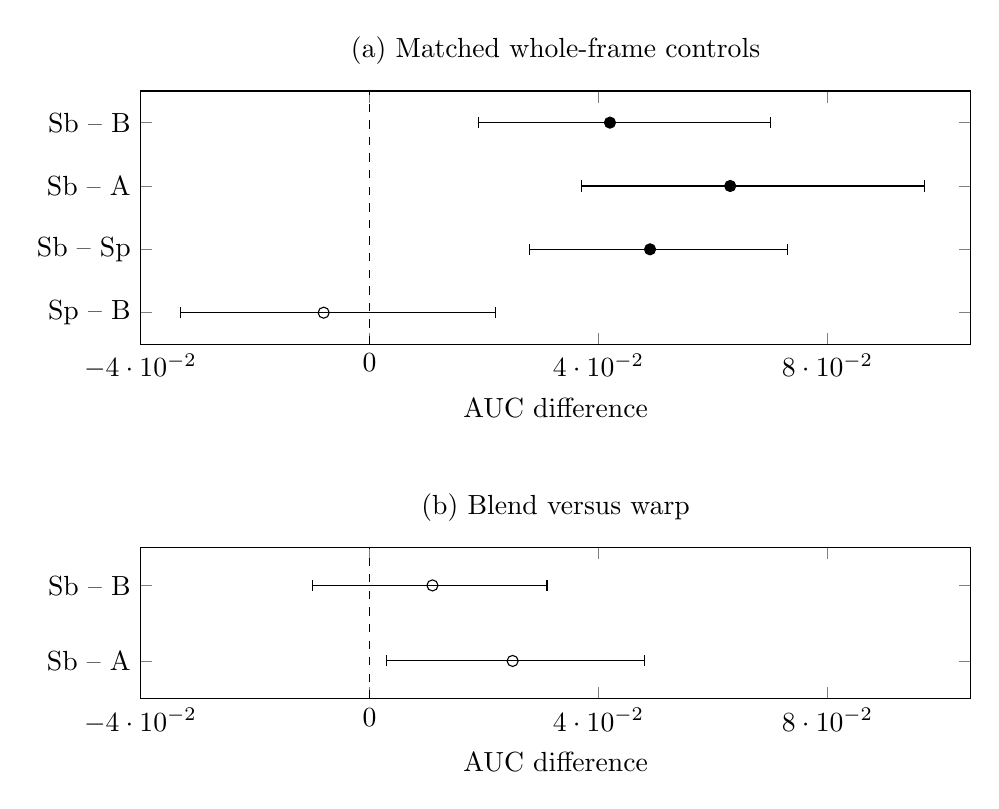
\begin{tikzpicture}
\begin{axis}[width=\linewidth,height=4.8cm,at={(0,0cm)},anchor=north west,scale only axis=false,title={(a) Matched whole-frame controls},xmin=-0.04,xmax=0.105,ymin=0.5,ymax=4.5,xtick={-0.04,0,0.04,0.08},xlabel={AUC difference},ytick={4,3,2,1},yticklabels={Sb -- B,Sb -- A,Sb -- Sp,Sp -- B}]
\addplot[dashed,mark=none] coordinates {(0,0.5) (0,4.5)};
\addplot[only marks,mark=*,error bars/.cd,x dir=both,x explicit] coordinates {(0.042,4) += (0.028000,0) -= (0.023000,0)};
\addplot[only marks,mark=*,error bars/.cd,x dir=both,x explicit] coordinates {(0.063,3) += (0.034000,0) -= (0.026000,0)};
\addplot[only marks,mark=*,error bars/.cd,x dir=both,x explicit] coordinates {(0.049,2) += (0.024000,0) -= (0.021000,0)};
\addplot[only marks,mark=o,error bars/.cd,x dir=both,x explicit] coordinates {(-0.008,1) += (0.030000,0) -= (0.025000,0)};
\end{axis}
\begin{axis}[width=\linewidth,height=3.5cm,at={(0,-5.8cm)},anchor=north west,scale only axis=false,title={(b) Blend versus warp},xmin=-0.04,xmax=0.105,ymin=0.5,ymax=2.5,xtick={-0.04,0,0.04,0.08},xlabel={AUC difference},ytick={2,1},yticklabels={Sb -- B,Sb -- A}]
\addplot[dashed,mark=none] coordinates {(0,0.5) (0,2.5)};
\addplot[only marks,mark=o,error bars/.cd,x dir=both,x explicit] coordinates {(0.011,2) += (0.020000,0) -= (0.021000,0)};
\addplot[only marks,mark=o,error bars/.cd,x dir=both,x explicit] coordinates {(0.025,1) += (0.023000,0) -= (0.022000,0)};
\end{axis}
\end{tikzpicture}
